\documentclass[a4paper, 11pt]{article}
\usepackage{comment} % enables the use of multi-line comments (\ifx \fi) 
\usepackage[top = 0.5in, bottom=0.5in]{geometry}
\usepackage{color, listings, graphicx,float, booktabs, tabularx, multirow, amsmath}
\usepackage[colorlinks=true, urlcolor=blue]{hyperref}

\definecolor{codegreen}{rgb}{0,0.6,0}
\definecolor{codegray}{rgb}{0.5,0.5,0.5}
\definecolor{codepurple}{rgb}{0.58,0,0.82}
\definecolor{backcolour}{rgb}{0.95,0.95,0.92}
 
\lstdefinestyle{mystyle}{
    backgroundcolor=\color{backcolour},   
    commentstyle=\color{codegreen},
    keywordstyle=\color{magenta},
    numberstyle=\tiny\color{codegray},
    stringstyle=\color{codepurple},
    basicstyle=\footnotesize,
    breakatwhitespace=false,         
    breaklines=true,                 
    captionpos=b,                    
    keepspaces=true,                 
    numbers=left,                    
    numbersep=5pt,                  
    showspaces=false,                
    showstringspaces=false,
    showtabs=false,                  
    tabsize=2
}
\lstset{style=mystyle}

\begin{document}
\graphicspath{{./figures/}}
\noindent
\large\textbf{Kyle Salitrik (kps168)} \\
\normalsize STAT 462\\
\large{Homework 1 Report} \hfill 

%%%%%%%%%%%%%%%%%%%%%%%%%%%%%%%%%%%%%%%%%%%%%%%%%%%%%%%%%%%%%%%%%%%%
%%% SECTION: Theoretical
%%%%%%%%%%%%%%%%%%%%%%%%%%%%%%%%%%%%%%%%%%%%%%%%%%%%%%%%%%%%%%%%%%%%


\section*{Theoretical Solutions}
\subsection*{Proof 1}
We know the properties:
\begin{flalign*}
	\beta_0 + \beta_1x_i  &= \hat{y_i} &\\
	y_i - \hat{y_i} &= \hat{\epsilon} &
\end{flalign*}
Using these identities and starting from the normal equations, we can show the following
\begin{flalign*}
	\sum_{i=1}^{n} y_i = \sum_{i=1}^{n} \beta_0 + \beta_1x_i &\rightarrow \sum_{i=1}^{n} y_i -\beta_0 + \beta_1x_i = 0 &\\
	\sum_{i=1}^{n} y_i - \hat{y_i} = 0 &\rightarrow \sum_{i=1}^{n} \hat{\epsilon_i} = 0 &
\end{flalign*}

\subsection*{Proof 2}
From the first equation in the last line above, we can see that:
\begin{flalign*}
	\sum_{i=1}^{n} y_i - \hat{y_i} = 0 \text{\quad So, necessarily: \quad} \sum_{i=1}^{n} y_i = \hat{y_i} &&
\end{flalign*}

\subsection*{Proof 3}

\begin{flalign*}
	\sum_{i=1}^{n} y_i &= \sum_{i=1}^{n} \beta_0 + \beta_1x_i &\\
	\sum_{i=1}^{n} y_i &= n\beta_0 + \beta_1\sum_{i=1}^{n} x_i &\\		
	\frac{1}{n}[\sum_{i=1}^{n} y_i] &= \frac{1}{n}[n\beta_0 + \beta_1\sum_{i=1}^{n} x_i] &\\	
	\bar{y} &= \beta_0 + \beta_1\bar{x} &
\end{flalign*}

\subsection*{Proof 4}
\begin{flalign*}
	SSE(b_0) & = (\sum_{i=1}^{n}y - nb_0)^2 &\\
	\frac{d}{db_0}SSE(b_0) &= 2n(\sum_{i=1}^{n}y - nb_0) = 0 &\\
	\sum_{i=1}^{n}y = nb_0 &\rightarrow \bar{y} = b_0 &
\end{flalign*}

%%%%%%%%%%%%%%%%%%%%%%%%%%%%%%%%%%%%%%%%%%%%%%%%%%%%%%%%%%%%%%%%%%%%
%%% SECTION: Applied
%%%%%%%%%%%%%%%%%%%%%%%%%%%%%%%%%%%%%%%%%%%%%%%%%%%%%%%%%%%%%%%%%%%%
\section*{Applied Analysis}
\subsection*{Part A: Data Correctness}
Starting with the 252 initial samples, if we re-calculate the body-fat percentage for each sample and normalizing any negative values to 0 and clipping the maximum value to 100 percent, we find that the provided data is incorrect for 35 samples. After assigning these new values and examining the data further, potential incorrect values for measurements are ruled out as follows.

\begin{itemize}
	\item Samples below 2\% and above 40\% body fat were excluded. The minimum was obtained through the chart on the (\href{''https://www.acefitness.org/acefit/healthy-living-article/60/112/what-are-the-guidelines-for-percentage-of-body-fat-loss''}{\underline{ACE}}) website and maximum was set to limit outliers.
	\item The minimum height accepted was cut to be over 50 inches to remove outliers.
	\item The maximum weight was also clipped to be below 300 pounds. Although the outlier may have been legitimate, it could have also been an error.
\end{itemize}

These constraints reduced the data down to 246 samples.

\subsection*{Part B: Data Summaries and Graphs}
The table below lists the mean and standard deviation of the density, body fat percentage, weight, height and abdomen circumference. Following this are the histograms for the distribution of each variable. In most cases the distributions appear to be mostly bell-shaped, and symmetrically distributed. The weight, however seems to be skewed towards lower weights with a few outliers.
\begin{table}[H]
	\centering
	\begin{tabular}{| c | c | c | c | c | c |}
		\hline
		          & Density & Body Fat & Weight & Height & Abdomen Circumference \\ \noalign{\hrule height 1.5pt}
		Mean      & 1.056   & 19.10    & 178.2  & 70.33  & 92.30                 \\ \hline
		Std. Dev. & 0.02    & 7.96     & 26.49  & 2.54   & 9.94                  \\ \hline
	\end{tabular}
\end{table}

Performing a p-value test on both the weight and body fat percentage, there is significant evidence that the average values for the greater population are 180 pounds and 20\% body fat, respectively.

\begin{figure}[H]
	\centering
	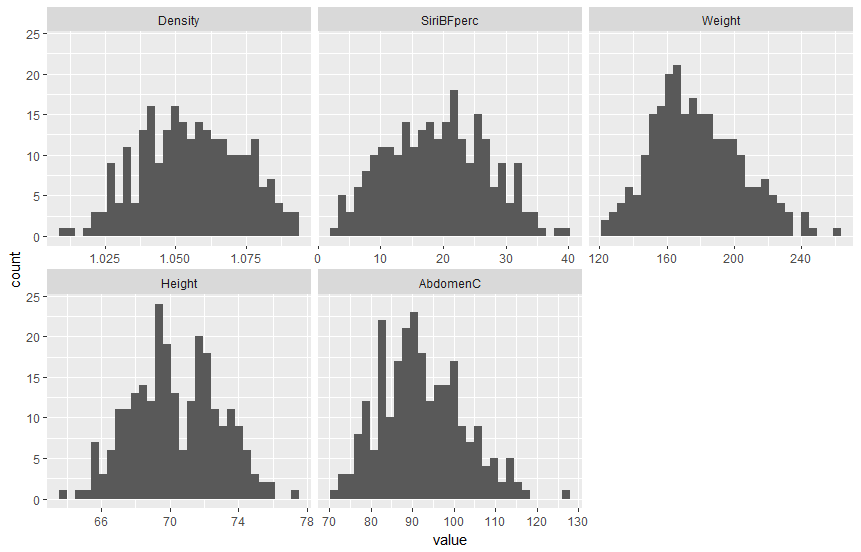
\includegraphics[width=\textwidth]{histograms.png}
\end{figure}

\subsection*{Part C: Linear Models}
For all linear models in this section the following model was used to fit the line to the data, where X represents the predictor used, Y represents the body fat percentage, and $\beta_0$ and $\beta_1$ represent the linear values that must be fit to the data.
\begin{equation}
Y = \beta_0 + \beta_1 X
\end{equation}

For the first model, we looked at the ability of weight to predict the amount of body fat. In this model, it can be seen that there is a positive correlation between the body fat percentage and the weight of the subject. For every pound of weight, we can expect about 0.18\% more body fat on the subject.
\begin{align*}
	&\beta_0 = -13.3064644 ,\quad \beta_1 = 0.1818511 ,\quad \sigma^2 =  40.38138 \\
	&\hat{y} = -13.3064644 + 0.1818511 x
\end{align*}
\begin{figure}[H]
	\centering
	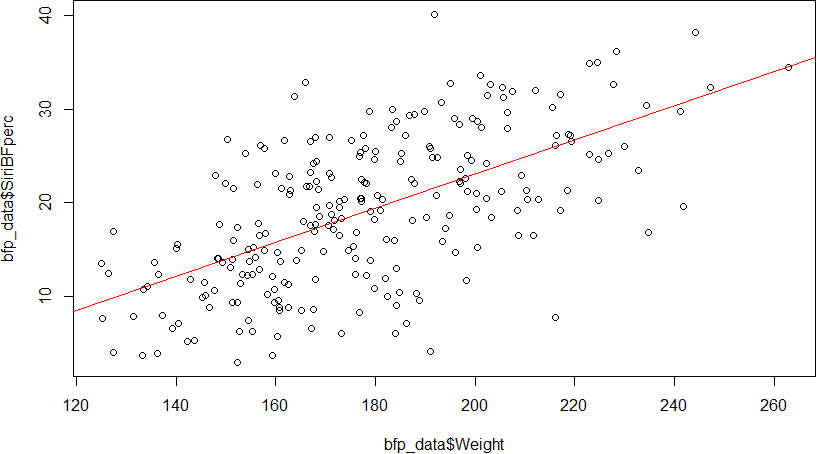
\includegraphics[scale=0.65]{weight_plot.png}
\end{figure}

Second, we examined the linearity between height and body fat percentage. In contrast to the weight, the height of the subject has a negative relationship with the body fat percentage as one might expect. For every inch in height we can observe a reduction of about 0.05 percent body fat.
\begin{align*}
	&\beta_0 = 22.58479808 ,\quad \beta_1 = -0.04960321 ,\quad \sigma^2 =  63.66048 \\
	&\hat{y} = 22.58479808 - 0.04960321 x
\end{align*}
\begin{figure}[H]
	\centering
	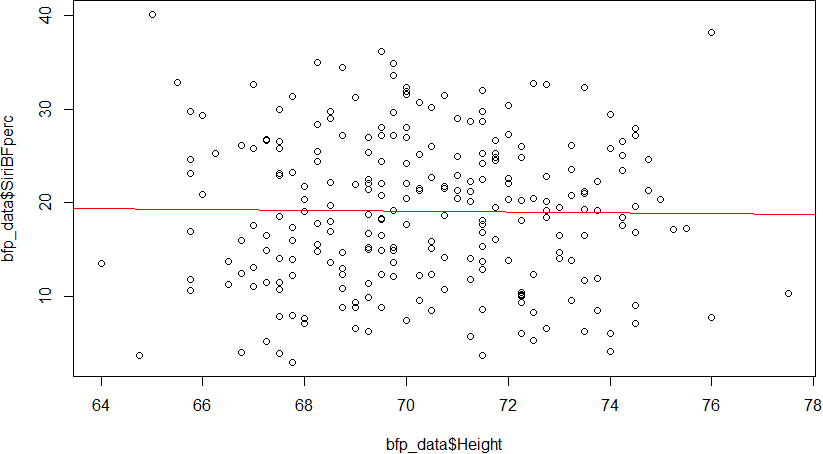
\includegraphics[scale=0.65]{height_plot.png}
\end{figure}

Finally, the abdomen circumference was used to fit a prediction of body fat. As one might expect, this model had the largest body fat percentage increase per unit of measurement increase. For each extra centimeter measured in abdomen circumference, we can expect an increase in body fat of about 0.65\%.
\begin{align*}
	&\beta_0 = -41.0361197 ,\quad \beta_1 = 0.6514835 ,\quad \sigma^2 =  21.60823 \\
	&\hat{y} = -41.0361197 + 0.6514835 x
\end{align*}
\begin{figure}[H]
	\centering
	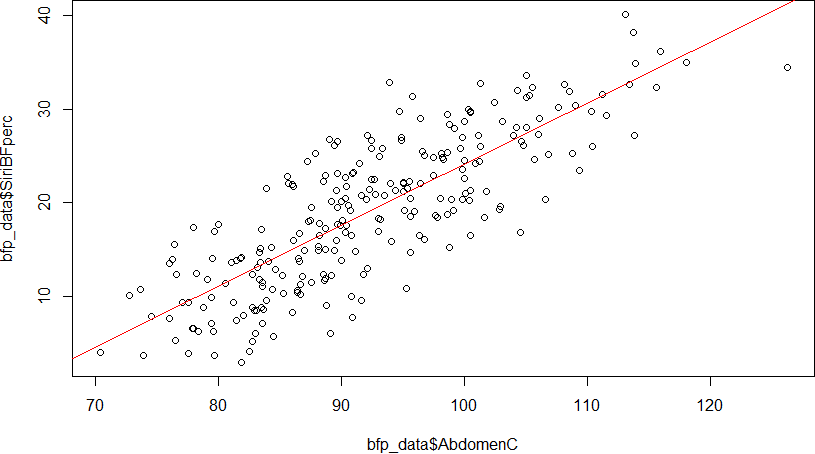
\includegraphics[scale=0.65]{abdomen_plot.png}
\end{figure}

We can look at the values of the coefficients of determination (correlation between the predictor and response) for each variable: 0.3658 for weight, 0.0002504 for height, and 0.6607 for abdomen circumference. higher values mean a more significant correlation between the predictor and response. It can be seen that our intuition is correct for the abdomen measurement being the most significant predictor of body fat percentage from the three variables examined.

\subsection*{Part D: New Predictor Model}
If we use common logic, a shorter person who weighs the same as a taller person would most likely be expected to have a higher body fat percentage. Therefore, it may be advantageous to examine the ratio of weight to height (weight/height, noted as np) vs the body fat percentage.
\begin{align*}
	&\beta_0 = -21.447564 ,\quad \beta_1 = 16.02598 ,\quad \sigma^2 =  34.11227 \\
	&\hat{y} = -21.447564 + 16.02598 x
\end{align*}
\begin{figure}[H]
	\centering
	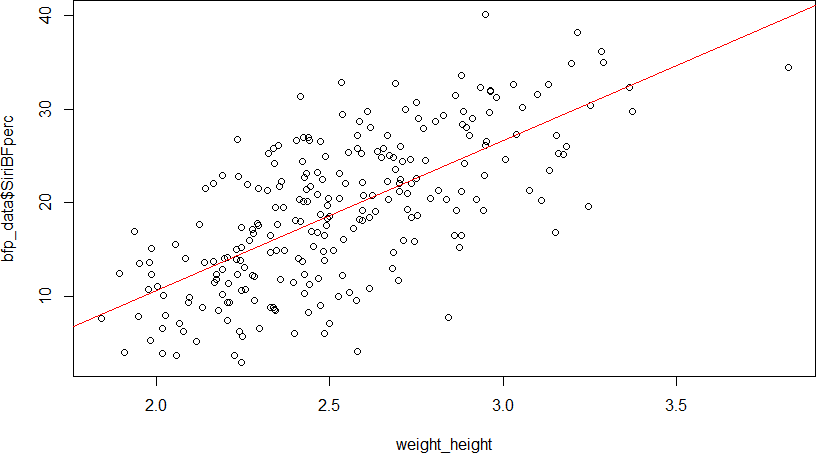
\includegraphics[scale=0.65]{np_plot.png}
\end{figure}
We can see that there is a stronger correlation between this ratio than either weight or height alone (with a coefficient of determination of 0.4643). However, the abdomen circumference is still a stronger predictor on it's own than using the ratio of weight to height.

\subsection*{Part E: Weight/Height vs Abdomen Circumference}
Finally, if we look at the linear model of between the weight to height and the abdomen circumference, we can find that the correlation between the ratio of height to weight and the abdomen circumference is about .8443.
\begin{align*}
	&\beta_0 = -0.36035408,\quad \beta_1 = 0.03131326 ,\quad \sigma^2 =  0.01792486 \\
	&\hat{y} = -0.36035408 + 0.03131326 x
\end{align*}
\begin{figure}[H]
	\centering
	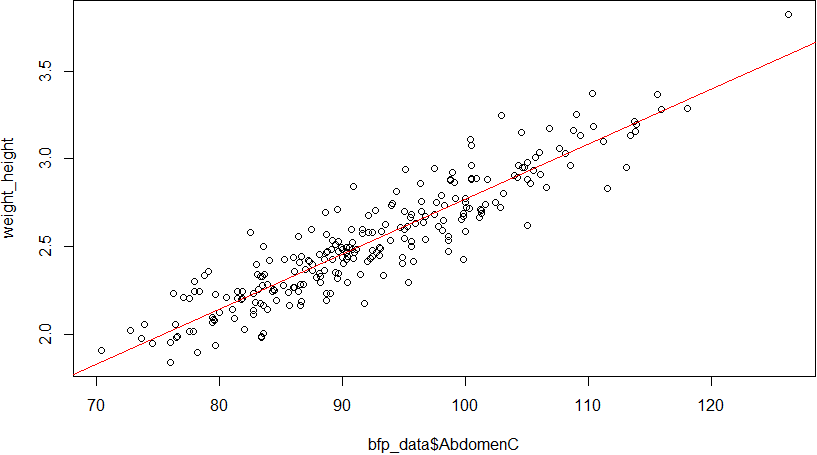
\includegraphics[scale=0.65]{ab_np_plot.png}
\end{figure}
With a near 100\% correlation, we can come to the conclusion that for the most part, both estimates seem to be estimates for the same information. In this case, that information is body fat percentage. If the correlation were significantly smaller, we could potentially be trying to predict the wrong type of information with either (or both) predictors.



%%%%%%%%%%%%%%%%%%%%%%%%%%%%%%%%%%%%%%%%%%%%%%%%%%%%%%%%%%%%%%%%%%%%
%%% SECTION: CODE APPENDIX
%%%%%%%%%%%%%%%%%%%%%%%%%%%%%%%%%%%%%%%%%%%%%%%%%%%%%%%%%%%%%%%%%%%%

% \newpage
% \section*{Code Appendix}
% \lstinputlisting[language=R]{../hw1.r}

\end{document}